\section{Benchmark NIST-5 "Battery"}
\label{sec:bench-5}

This is a heat conduction problem in a nonhomogeneous material. It comes with an anisotropic solution and
multiple singularities. The solution has multiple point singularities in the interior of the domain.
The equation solved is given by
\begin{equation} \label{heat-conduction}
-\frac{\partial }{\partial x}\left(p(x, y)\frac{\partial u}{\partial x}\right)
-\frac{\partial }{\partial y}\left(q(x, y)\frac{\partial u}{\partial y}\right) = f,
\end{equation}
in the domain $\Omega = (0, 8.4) \times (0, 24)$, equipped with zero Neumann boundary condition on the left edge, Natural boundary conditions on the rest of the boundary:

\begin{equation}
p(x, y)\frac{\partial u}{\partial x}\nu_1 + q(x, y)\frac{\partial u}{\partial y}\nu_2 = g_{left}(x, y) \ \mbox{on} \  \Gamma_{left}
\end{equation}

\begin{equation}
p(x, y)\frac{\partial u}{\partial x}\nu_1 + q(x, y)\frac{\partial u}{\partial y}\nu_2 + c(x, y)u = g_{right}(x, y) \ \mbox{on} \ \Gamma_{right}
\end{equation}

\begin{equation}
p(x, y)\frac{\partial u}{\partial x}\nu_1 + q(x, y)\frac{\partial u}{\partial y}\nu_2 + c(x, y)u = g_{top}(x, y) \ \mbox{on} \ \Gamma_{top}
\end{equation}

\begin{equation}
p(x, y)\frac{\partial u}{\partial x}\nu_1 + q(x, y)\frac{\partial u}{\partial y}\nu_2 + c(x, y)u = g_{bottom}(x, y) \ \mbox{on} \ \Gamma_{bottom},
\end{equation}
where $p(x, y)$, $q(x, y)$, $c(x, y)$, $g(x, y)$, and the right hand side $f$ are constant functions (different in respective materials).

The solution of NIST-5 is shown in Fig. \ref{fig:sln-nist05}.
\begin{figure}[!ht]
\centering
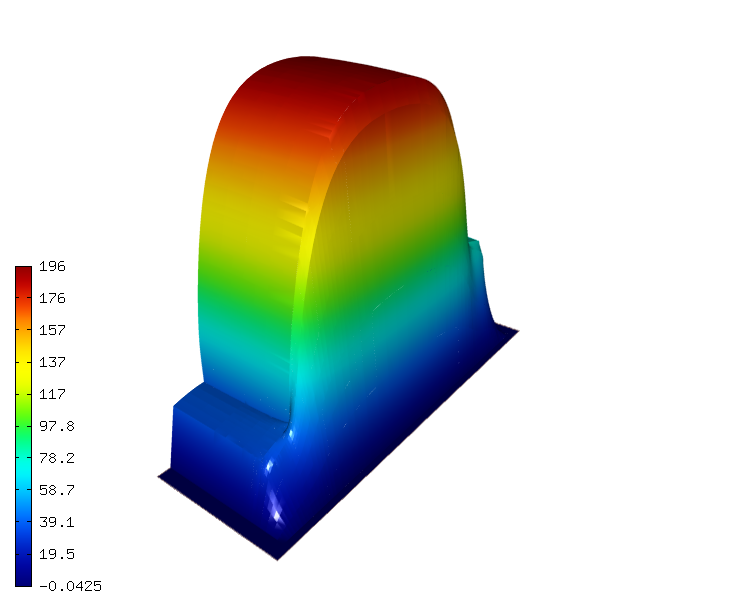
\includegraphics[height=35mm]{nist/nist-5/solution-3d.png}
\caption{The solution to NIST-5 benchmark problem.}
\label{fig:sln-nist05}
\end{figure}
